\label{sec:data}
% Main characteristics of the data set: source, type of data
% Description of variables used for the	analysis and correspondence with the (ideal) magnitudes in the empirical specification
% Descriptive statistics of the	main variables in the analysis
We have scraped most of our data from various web sources in respect of the terms of use. The descriptive statistics for the main variables are shown in Table \ref{tab:descriptive} and described in further detail for the remainder of this section.
\par
For the regressions we log-transform electricity consumption, the number of electricity meters, and the electricity spot price. Before taking the natural logarithm the variables are censored with $1$ as the lower bound whereby we loose some information as the spot price is negative for a few instances due to exceed wind power production.
\begin{table}[H]
  \centering
  \caption{Descriptive statistics}
  \label{tab:descriptive}
  \footnotesize
    \begin{tabular}{l*{1}{ccccc}}
\hline\hline
                    &\multicolumn{5}{c}{}                                            \\
                    &        mean&          sd&         min&         p50&         max\\
\midrule
Wholesale electricity consumption, MWh&    34.17217&     83.3248&     .063157&      5.9281&    757.5571\\
Retail electricity consumption, MWh&    28.74596&    74.08786&           0&    5.833275&    906.3964\\
Number of wholesale meters&    923.9638&    2440.423&           7&       140.5&       17674\\
Number of retail meters&    57551.23&      148260&         858&       14371&     1006061\\
- of which flex-settled&    4299.473&    37193.14&           0&           0&      596267\\
- of which residual &    53251.75&    134556.1&         855&       14357&      998864\\
Electricity spot price, DKK&    252.9863&    108.0154&     -398.61&      234.94&      1898.9\\
Wind power prognosis for DK1, GWh&    1.225359&    .9221094&           0&       1.002&       3.973\\
Wind power prognosis for DK2, GWh&    .3266759&    .2702798&           0&        .249&       1.084\\
wp                  &    1.075578&    .9126432&           0&        .796&       3.973\\
wp\_other            &    .4764563&    .5610359&           0&         .31&       3.973\\
Wind power prognosis for Sweden, GWh&    1.862874&    1.118507&        .062&       1.668&        5.84\\
Price region DK1 (Western Denmark)&    .8333333&    .3726781&           0&           1&           1\\
Share time-of-use tariff&    .0001378&    .0079703&           0&           0&    .5926748\\
Temperature         &    9.094615&    6.915881&       -11.9&         8.7&        31.4\\
Daytime             &    .5135309&    .4857462&           0&    .6666667&           1\\
Time trend          &    547.4559&    316.4119&           0&         547&        1095\\
Holiday (not in a weekend)&    .0437643&    .2045702&           0&           0&           1\\
\midrule
Observations        &     1420200&            &            &            &            \\
\bottomrule\end{tabular}

\end{table}

\subsection{Grid-level consumption}
\label{subsec:d_consumption}
The Danish Transmission System Operator (TSO), Energinet provides public access to hourly aggregated consumption data\footnote{Scraped from \href{https://www.energidataservice.dk/en/dataset/consumptionpergridarea/}{energidataservice.dk/en/dataset/consumptionpergridarea} using their transparent API via SQL statements.} since January 2016 for each grid company grouped by hourly-settled consumption, flex settled consumption, and residual consumption. This allows us to distinguish between wholesale and retail consumption. Hourly-settled consumption consists of all firms with an annual electricity consumption of at least 100,000 kWh. Flex-settled consumption was introduced in January 2018 such that households and small firms can also have their electricity consumption settled flexibly according to hour-by-hour prices. Though installation of smart meters to enable flex-settling is only being introduced gradually, this allows a portion of residential consumers and small firms to respond to price changes at an hourly rather than a yearly or quarterly basis. The residual consumption is the remaining retail electricity consumption for which flex-settling is not used, thus, including all households and small firms till December 1 2017 and a majority throughout 2018 as well.
\begin{figure}[H]
  \centering
  \caption{Mean electricity consumption by hour and type}
    \label{fig:cons_hours}
  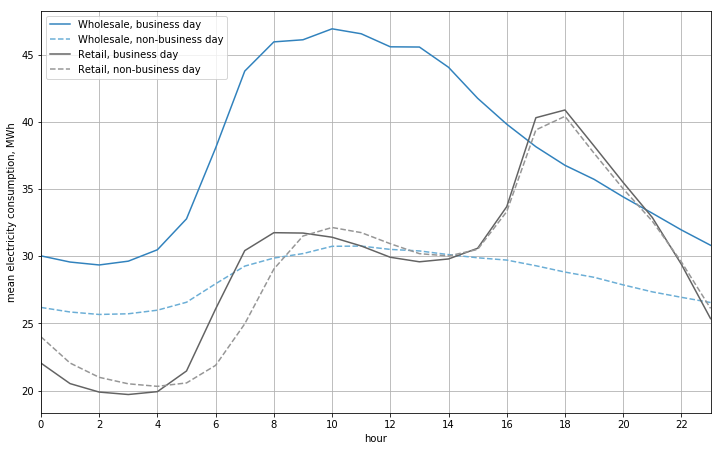
\includegraphics[width=1 \textwidth]{03_figures/cons_hours}
\end{figure}

\begin{figure}[H]
  \centering
  \caption{Time series for mean electricity consumption (business days)}
  \label{fig:cons_time_series}
  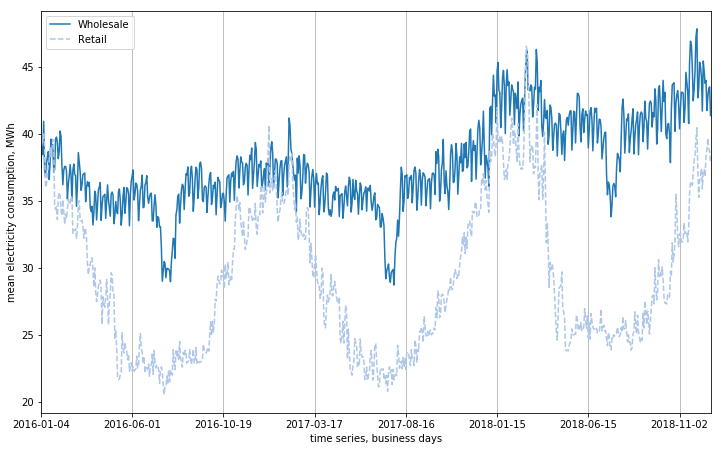
\includegraphics[width=1 \textwidth]{03_figures/cons_time series, business days}
\end{figure}
\noindent
As shown in figure \ref{fig:cons_hours} and \ref{fig:cons_time_series} both wholesale and retail consumption follow clear patterns not only within the day but also between days and across the year. That is, wholesale consumption is at its lowest on weekends and bank holidays as well as during the summer holiday while retail consumption peaks for the hours 5-7 PM (from here written as hours 17-19) and during the winter half of the year.
\medskip\\
For each grid we include the number of metering points\footnote{Received from Energinet after request.} by each of the three consumer categories. This data is monthly by the \nth{1} of the month. For studies on state-level data it is likewise common to control for size \citep{burke2017price}.
\par
The landscape of grid companies have changed drastically. From consisting of 74 grid companies by early 2016, only 56 grid companies remained by the end of 2018 (see figure \ref{fig:elnetgraenser} in appendix \ref{app:grids}). Removing the two grids with less than 10 metering points and the six grids with no wholesale consumption leaves us with 48 grids of which no less than 39 are located in Western Denmark. For a merged grid company we apply the sum of grids included in a future merge to each prior month as described in appendix \ref{app:grids}.


\subsection{Spot market prices and wind power prognosis}
\label{subsec:d_spot}
We include the hour-by-hour spot market price on the day-ahead-market for the price region DK1 (Western Denmark) or DK2 (Eastern Denmark) depending on where the grid company is located (see section \ref{sec:theory}). An important factor for the spot price on the day-ahead-market is the hour-by-hour wind power prognosis for the following day.\footnote{'Elspot prices' and 'Wind power prognosis' by price region and year is updated daily after 2PM by Nord Pool and downloadable at \href{https://www.nordpoolgroup.com/historical-market-data/}{nordpoolgroup.com/historical-market-data}} While being less volatile than wind power production, price is nonetheless highly volatile from day to day while having increased in 2018 as illustrated by the time series in figure \ref{fig:wp_dk1_time_series} and \ref{fig:wp_dk2_time_series} (appendix \ref{app:data}).
\par
The wind power prognosis first and foremost takes into account weather forecasts in relation to the positions and capacity of windmills but also takes into account the expected demand as some wind mills can possibly be turned off if the expected price is too low. However, except for a slight peak in the afternoon and evening that is more likely due to sea and land breezes, wind power does not seem to care much for consumption patterns during the day (figure \ref{fig:trio_DK2_hours} for DK2 and \ref{fig:wp_dk1_hours} for DK1) and especially not across weekdays (figure \ref{fig:wp_price_weekday}).
\par
On the contrary, the daily pattern of the spot price on average follows the pattern of demand by and large. The biggest gap between price and total consumption seen in figure \ref{fig:trio_DK2_hours} occurs during the afternoon where the low price relative to demand could possibly be explained by the higher wind power production.
\begin{figure}[H]
  \centering
  \caption{Total consumption, wind power and spot price by hour (business days)}
  \label{fig:trio_DK2_hours}
    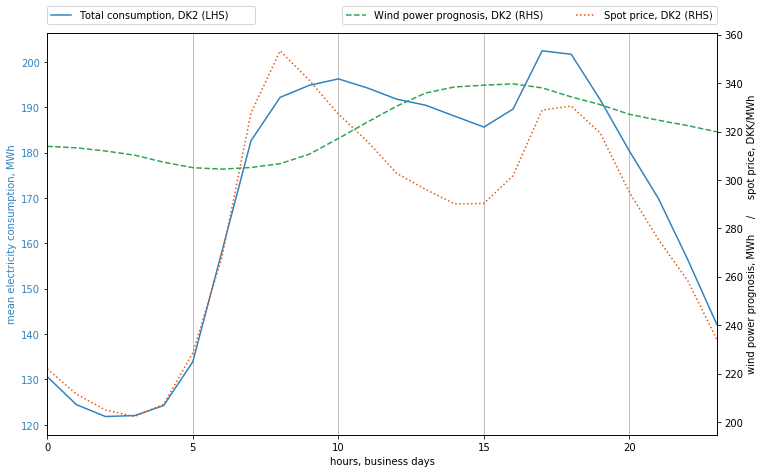
\includegraphics[width=1 \textwidth]{03_figures/trio_DK2_hours, business days}
\end{figure}


\subsection{Time-of-use tariff}
\label{subsec:d_tout}
From December 2017 grid companies have been allowed to introduce time-of-use (TOU) tariffs for retail consumption in order to send signals that can direct the more flexible tasks away from the peak hours around dinnertime. Thus, two of the bigger grid companies have already introduced TOU tariffs for the peak-hours 17-19 for the months October-March in which electricity consumption is also higher due to the lack of daylight. While Konstant initially only runs an experiment for a smaller group of flex-settled consumers, Radius is introducing a full-scale TOU tariff scheme while exchanging the old prepayment meters with smart meters for the 600,000 retail customers in the Copenhagen metropolitan area.\footnote{See \href{https://ing.dk/artikel/nu-loebes-fleksible-elforbrug-omsider-gang-209251}{ing.dk/artikel/nu-loebes-fleksible-elforbrug-omsider-gang-209251} (Danish).}
\par
The variable for the TOU tariff represents the share of retail customers in Radius exposed to the tariff. As seen in Figure \ref{fig:radius_w39_w40} and Table \ref{tab:descriptive} below the increasing share ends near 60 pct. in December 2018. The concept of aggregate data makes it difficult to demarcate changes in behavior from changes in composition. In figure \ref{fig:radius_w39_w40} we try to investigate the discontinuity around October 1 2018 as week 39 is in September and week 40 is in October. From a graphical inspection no clear response to the TOU tariff stands out, except that flex-settled consumers have higher consumption during the day and residual consumers during the night which might be due to sociodemographic differences between the areas with smart meters and those where it has yet to be implemented.
\begin{figure}[H]
  \centering
  \caption{Flex-settled and residual consumption by week (Radius, 2018)}
  \label{fig:radius_w39_w40}
      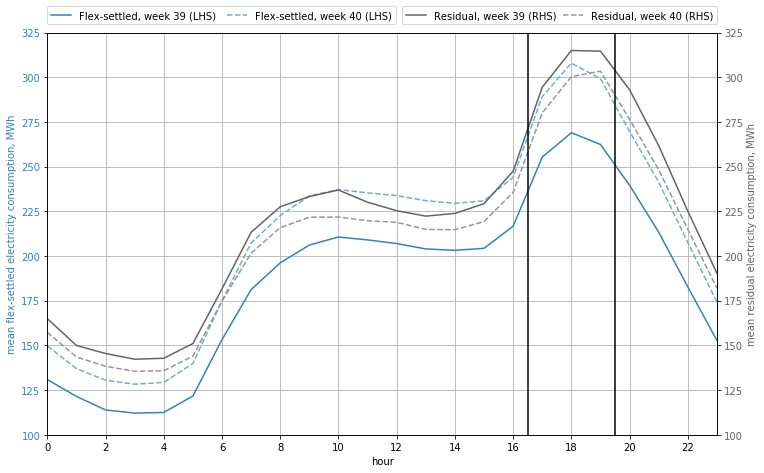
\includegraphics[width=1 \textwidth]{03_figures/radius_w39_w40}
\end{figure}

\subsection{Weather data}
\label{subsec:d_weather}
The outside temperature is relevant to the extent that electrical heaters or air conditioning is used \citep{lijesen2007real, vesterberg2014residential}. As the electricity consumption ceteris paribus is expected to be higher for both low-end and high-end temperatures, we let the effect of temperature enter as a \nth{2} order polynomial in the estimation of electricity consumption.\footnote{Scraped via iterative lookups in the records of the Danish Meteorological Institute at \href{https://www.dmi.dk/vejrarkiv/}{dmi.dk/vejrarkiv/}}
\medskip\\
Lighting is used more in the absence of daylight. Therefore, an indicator for daytime is included such that $daytime=1$ for hours between sunrise and sunset and e.g. $daytime=0.25$ for $hour=7$ if sunrise was a quarter past 7.\footnote{Sunrise and sunset are scraped for each date in the sample via iterative lookups at \href{https://soltider.dk/}{soltider.dk}}
\medskip\\
Taking advantage of the dense size of Denmark, temperature and daytime are not scraped by the location of each of the 52 grid companies which often cross municipality-borders but for the two most populace municipalities and applied to all grids within that price region.\footnote{Temperature is for the municipalities of Aarhus and Copenhagen respectively while sunrise and sunset are for the City Hall Square in each of the two cites.}

\subsection{Time variables}
\label{subsec:d_time}
Year dummies as well as a time trend indicating the number of days since January 1 2016 are included to account for economic growth (increase in electricity consumption), technological progress (decrease in electricity consumption) \citep{lijesen2007real}, or compositional changes that can affect electricity consumption other than the number of meters.
\medskip\\
Danish bank holidays as well as a few other common holidays with lower wholesale electricity consumption\footnote{January 2 (the day after New Year's Day), May 1 (International Workers' Day), Friday after Ascension Day, June 5 (Constitution Day), last Friday before Christmas, and the days between Christmas and New Year's. All holidays according to \href{https://kalendersiden.dk/}{kalendersiden.dk}} are taken into account in order to do sample split regressions for business days and non-business days, the latter including holidays and weekends.
